\documentclass{article}

\usepackage{fancyhdr}
\usepackage{extramarks}
\usepackage{amsmath}
\usepackage{amsthm}
\usepackage{amsfonts}
\usepackage{tikz}
\usepackage[plain]{algorithm}
\usepackage{algpseudocode}

\usetikzlibrary{automata,positioning}

%
% Basic Document Settings
%

\topmargin=-0.45in
\evensidemargin=0in
\oddsidemargin=0in
\textwidth=6.5in
\textheight=9.0in
\headsep=0.25in

\linespread{1.1}

\pagestyle{fancy}
\lhead{\hmwkAuthorName}
\chead{\hmwkClass\ (\hmwkClassInstructor\ \hmwkClassTime): \hmwkTitle}
\rhead{\firstxmark}
\lfoot{\lastxmark}
\cfoot{\thepage}

\renewcommand\headrulewidth{0.4pt}
\renewcommand\footrulewidth{0.4pt}

\setlength\parindent{0pt}

%
% Create Problem Sections
%

\newcommand{\enterProblemHeader}[1]{
    \nobreak\extramarks{}{Problem \arabic{#1} continued on next page\ldots}\nobreak{}
    \nobreak\extramarks{Problem \arabic{#1} (continued)}{Problem \arabic{#1} continued on next page\ldots}\nobreak{}
}

\newcommand{\exitProblemHeader}[1]{
    \nobreak\extramarks{Problem \arabic{#1} (continued)}{Problem \arabic{#1} continued on next page\ldots}\nobreak{}
    \stepcounter{#1}
    \nobreak\extramarks{Problem \arabic{#1}}{}\nobreak{}
}

\setcounter{secnumdepth}{0}
\newcounter{partCounter}
\newcounter{homeworkProblemCounter}
\setcounter{homeworkProblemCounter}{1}
\nobreak\extramarks{Problem \arabic{homeworkProblemCounter}}{}\nobreak{}

%
% Homework Problem Environment
%
% This environment takes an optional argument. When given, it will adjust the
% problem counter. This is useful for when the problems given for your
% assignment aren't sequential. See the last 3 problems of this template for an
% example.
%
\newenvironment{homeworkProblem}[1][-1]{
    \ifnum#1>0
        \setcounter{homeworkProblemCounter}{#1}
    \fi
    \section{Problem \arabic{homeworkProblemCounter}}
    \setcounter{partCounter}{1}
    \enterProblemHeader{homeworkProblemCounter}
}{
    \exitProblemHeader{homeworkProblemCounter}
}

%
% Homework Details
%   - Title
%   - Due date
%   - Class
%   - Section/Time
%   - Instructor
%   - Author
%

\newcommand{\hmwkTitle}{Homework 2}
\newcommand{\hmwkDueDate}{February 5, 2019}
\newcommand{\hmwkClass}{Physics 216}
\newcommand{\hmwkClassTime}{Section 509}
\newcommand{\hmwkClassInstructor}{Professor Ostrovskya}
\newcommand{\hmwkAuthorName}{\textbf{Amari West}}
\newcommand{\hmwkDueTime}{11:59pm}
\newcommand{\hmwkPages}{Pages: 3}

%
% Title Page
%

\title{
    \vspace{2in}
    \textmd{\textbf{\hmwkClass:\ \hmwkTitle}}\\
    \normalsize\vspace{0.1in}\small{Due\ on\ \hmwkDueDate\ at \hmwkDueTime}\\
    \normalsize\vspace{0.1in} \hmwkPages \\
    \vspace{0.1in}\large{\textit{\hmwkClassInstructor\ \hmwkClassTime}}
    \vspace{3in}
}

\author{\hmwkAuthorName}
\date{}

\renewcommand{\part}[1]{\textbf{\large Part \Alph{partCounter}}\stepcounter{partCounter}\\}

%
% Various Helper Commands
%

% Useful for algorithms
\newcommand{\alg}[1]{\textsc{\bfseries \footnotesize #1}}

% For derivatives
\newcommand{\deriv}[1]{\frac{\mathrm{d}}{\mathrm{d}x} (#1)}

% For partial derivatives
\newcommand{\pderiv}[2]{\frac{\partial}{\partial #1} (#2)}

% Integral dx
\newcommand{\dx}{\mathrm{d}x}

% Alias for the Solution section header
\newcommand{\solution}{\textbf{\large Solution}}

% Probability commands: Expectation, Variance, Covariance, Bias
\newcommand{\E}{\mathrm{E}}
\newcommand{\Var}{\mathrm{Var}}
\newcommand{\Cov}{\mathrm{Cov}}
\newcommand{\Bias}{\mathrm{Bias}}

% Allow double underline
\def\doubleunderline#1{\underline{\underline{#1}}}

% Allow for units in math mode
\newcommand{\unit}[1]{\ensuremath{\, \mathrm{#1}}}

\begin{document}

\maketitle

\pagebreak

\begin{homeworkProblem}
	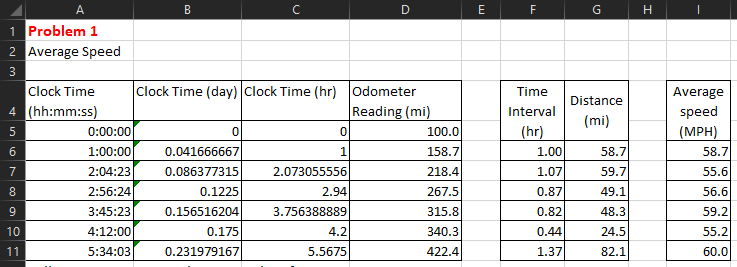
\includegraphics[scale=.75]{problem1}
\end{homeworkProblem}

\begin{homeworkProblem}
	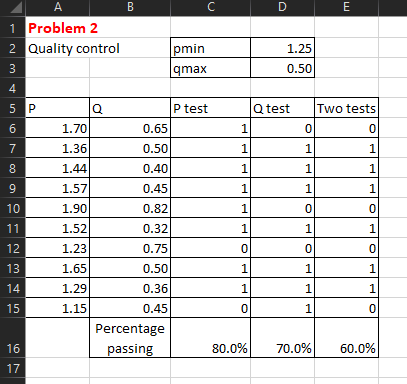
\includegraphics[scale=.75]{problem2}
	
	The following are listed equations within the specified cells.
	
	\begin{itemize}
		\item \textbf{D11} =IF(B11$<=$\$D\$3, 1, 0)
		
		\item \textbf{E11} =IF(AND(A11$>=$\$D\$2,B11$<=$\$D\$3), 1, 0)
		
		\item \textbf{D16} =IF(B6$<=$\$D\$3, 1, 0)
	\end{itemize}

	If $q_{max}$ is changed to 0.75 and $p_{min}$ is changed to 1.50, the passing rate for both tests and the $q$ test decrease while the $p$ test increases, as observed below.
	
	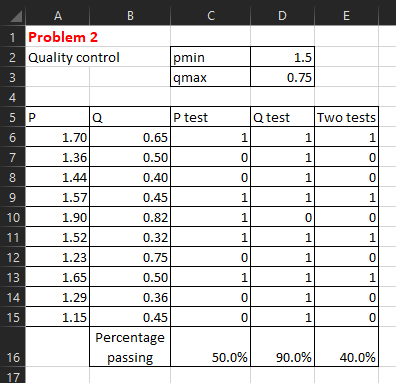
\includegraphics[scale=0.75]{problem2b}
	
\end{homeworkProblem}


\begin{homeworkProblem}

	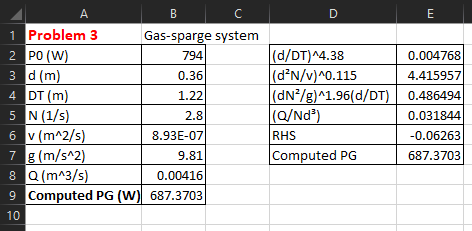
\includegraphics{problem3}
	
	\begin{itemize}
		\item \textbf{E2} =(B3/B4)\^{}4.38
		\item \textbf{E3} =(B3\^{}2*B5/B6)\^{}0.115
		\item \textbf{E4} =(B3*(B5\^{}2)/B7)\^{}(1.96*(B3/B4))
		\item \textbf{E5} =B8/(B5*B3\^{}3)
		\item \textbf{E7} =E2*E3*E4*E5*-192
		\item \textbf{B9} =B2 * 10\^{}(-192 * (B3/B4)\^{}4.38 * ((B3\^{}2 * B5) / B6)\^{}(0.115) * ((B3 * B5\^{}2) / B7)\^{}(1.96 * (B3 / B4)) * (B8 / (B5 * B3\^{}3)) )
	\end{itemize}


	
\end{homeworkProblem}




\end{document}
